\documentclass{scrreprt}

\usepackage{aligned-overset}
\usepackage{amsmath}
\usepackage{amsthm}
\usepackage{amssymb}
\usepackage{bm}
\usepackage[inline, shortlabels]{enumitem}
\usepackage{hyperref}
\usepackage[utf8]{inputenc}
\usepackage{listings}
\usepackage{multicol}
\usepackage{mathtools}
\usepackage{pdflscape}
\usepackage{physics}
\usepackage{polynom}
\usepackage{tabularx}
\usepackage[table]{xcolor}
\usepackage{titling}
\usepackage{fancyhdr}
\usepackage{xfrac}
\usepackage{pgfplots}

\pgfplotsset{compat = newest}
\usepgfplotslibrary{fillbetween}
\usetikzlibrary{arrows, arrows.meta}
\usetikzlibrary{calc}
\usetikzlibrary{patterns}

\author{Karsten Lehmann}
\date{WiSe 2024/25}
\title{Übungsblatt 9\\INF-B-110, Diskrete Strukturen}

\setlength{\parindent}{0pt}

\setlength{\headheight}{26pt}
\pagestyle{fancy}
\fancyhf{}
\lhead{\thetitle}
\rhead{\theauthor}
\lfoot{\thedate}
\rfoot{Seite \thepage}

\newcommand{\ggT}[0]{\text{ggT}}
\DeclarePairedDelimiter{\floor}{\lfloor}{\rfloor}

\begin{document}

\paragraph{Ü 9.1}
\begin{enumerate}[(a)]
\item Gegeben sind Graphen $G_1$ und $G_2$ durch die Diagramme:

  \begin{minipage}{.45\textwidth}
    \begin{tikzpicture}
      \node[circle, draw, inner sep=0pt, minimum size=1mm,label=below:{1}] (1) at (0,0) {};
      \node[circle, draw, inner sep=0pt, minimum size=1mm,label=below:{2}] (2) at (1,0) {};
      \node[circle, draw, inner sep=0pt, minimum size=1mm,label=right:{4}] (4) at ($(1.5, {sqrt(3)/2})$) {};
      \node[circle, draw, inner sep=0pt, minimum size=1mm,label=above:{6}] (6) at ($(1, {sqrt(3)})$) {};
      \node[circle, draw, inner sep=0pt, minimum size=1mm,label=above:{5}] (5) at ($(0, {sqrt(3)})$) {};
      \node[circle, draw, inner sep=0pt, minimum size=1mm,label=left:{3}] (3) at ($(-0.5, {sqrt(3)/2})$) {};

      \draw (1) -- (2) -- (4) -- (6) -- (1) -- (3) -- (5) -- (6);

      \node at (0.5, -1) {$G_1$};
    \end{tikzpicture}
  \end{minipage}
  \begin{minipage}{.45\textwidth}
    \begin{tikzpicture}
      \node[circle, draw, inner sep=0pt, minimum size=1mm,label=above:{1}] (1) at (0,0) {};
      \node[circle, draw, inner sep=0pt, minimum size=1mm,label=below:{2}] (2) at (0,-2) {};
      \node[circle, draw, inner sep=0pt, minimum size=1mm,label=below:{3}] (3) at (1,-2) {};
      \node[circle, draw, inner sep=0pt, minimum size=1mm,label=below:{4}] (4) at (2,-2) {};
      \node[circle, draw, inner sep=0pt, minimum size=1mm,label=above:{5}] (5) at (2,0) {};

      \draw (1) -- (2) -- (5) -- (4) -- (1) -- (3) -- (5);

      \node at (1, -3) {$G_2$};
    \end{tikzpicture}
  \end{minipage}

  \begin{enumerate}[(1)]
  \item Zeichnen Sie je ein Diagramm der Komplementgraphen beider Graphen.

    \subparagraph{Lsg.}\phantom{\null}

    \begin{minipage}{.45\textwidth}
      \begin{tikzpicture}
        \node[circle, draw, inner sep=0pt, minimum size=1mm,label=below:{1}] (1) at (0,0) {};
        \node[circle, draw, inner sep=0pt, minimum size=1mm,label=below:{2}] (2) at (1,0) {};
        \node[circle, draw, inner sep=0pt, minimum size=1mm,label=right:{4}] (4) at ($(1.5, {sqrt(3)/2})$) {};
        \node[circle, draw, inner sep=0pt, minimum size=1mm,label=above:{6}] (6) at ($(1, {sqrt(3)})$) {};
        \node[circle, draw, inner sep=0pt, minimum size=1mm,label=above:{5}] (5) at ($(0, {sqrt(3)})$) {};
        \node[circle, draw, inner sep=0pt, minimum size=1mm,label=left:{3}] (3) at ($(-0.5, {sqrt(3)/2})$) {};

        \draw (1) -- (4) -- (5) -- (1);
        \draw (6) -- (2) -- (3) -- (6);
        \draw (3) -- (4);
        \draw (5) -- (2);

        \node at (0.5, -1) {$G_1$};
      \end{tikzpicture}
    \end{minipage}
    \begin{minipage}{.45\textwidth}
      \begin{tikzpicture}
        \node[circle, draw, inner sep=0pt, minimum size=1mm,label=above:{1}] (1) at (0,0) {};
        \node[circle, draw, inner sep=0pt, minimum size=1mm,label=below:{2}] (2) at (0,-2) {};
        \node[circle, draw, inner sep=0pt, minimum size=1mm,label=above:{3}] (3) at (1,-1.7) {};
        \node[circle, draw, inner sep=0pt, minimum size=1mm,label=below:{4}] (4) at (2,-2) {};
        \node[circle, draw, inner sep=0pt, minimum size=1mm,label=above:{5}] (5) at (2,0) {};

        \draw (1) -- (5);
        \draw (2) -- (3) -- (4) -- (2);

        \node at (1, -3) {$G_2$};
      \end{tikzpicture}
    \end{minipage}


  \item Geben Sie für $G_1$ alle Wege vom Knoten 2 zum Knoten 5 an, sowie
    einen Kantenzug zwischen diesen Knoten, der kein Weg ist.

    \subparagraph{Lsg.} Die Wege sind
    \begin{itemize}
    \item $\qty\big{2, 1, 6, 5}$
    \item $\qty\big{2, 1, 3, 5}$
    \item $\qty\big{2, 4, 6, 5}$
    \item $\qty\big{2, 4, 6, 1, 3, 5}$
    \end{itemize}
  \end{enumerate}
  Ein Kantenzug, der kein Weg ist, wäre zum Beispiel
  $\qty\big{2, 1, 6, 4, 2, 1, 3, 5}$.

\newpage
\item Beweisen Sie, dass es keinen Graphen $G$ mit 6 Knoten gibt, der isomorph zu
  $\overline{G}$ ist.

  \subparagraph{Lsg.} Sei $V$ mit $\abs{V} = 6$,
  $E \subseteq \binom{V}{2}$ beliebig und $G = \qty\big(V, E)$.
  Dann ist $\overline{G} = \qty(V, \binom{V}{2} \setminus E)$.
  Es sind $G$ und $\overline{G}$ isomorph, wenn eine Bijektion
  $f \colon V \to V$ existiert mit
  \[
    \qty\big{u, v} \in E
    \iff \qty{f\qty\big(u), f\qty\big(v)} \in \binom{V}{2} \setminus E
  \]
  Nun ist $\abs{\binom{V}{2}} = \binom{\abs{V}}{2} = \binom{6}{2}
  = \frac{6!}{2!\qty\big(6 - 2)!} = \frac{720}{40} = 15$.
  Dementsprechend besitzen $G$ und $\overline{G}$ zusammen 15 Kanten und somit
  haben $G$ und $\overline{G}$ zwingend eine unterschiedliche Anzahl an Kanten.

  Somit hat immer einer der beiden Graphen eine Kante, die nicht durch die
  Bijektion auf die Kantenmenge des anderen Graphen abgebildet werden kann.

  Allgemein gesagt auch, damit zwei Graphen $G$ und $H$ isomorph sein können,
  muss zwingen $\abs{E\qty\big(G)} = \abs{E\qty\big(H)}$.
\end{enumerate}

\paragraph{Ü 9.2} Für $n \in \mathbb{N}, n > 0$ sei
$M_n \coloneqq \qty\big{1, 2, \ldots, 2n}$ und es sei
$G_n \coloneqq \qty(V_n, E_n)$ derjenige Graph, der durch
\begin{flalign*}
  V_n &\coloneqq \qty{A \subseteq M_n \:{\big|}\: \abs{A} = n}, \\
  E_n &\coloneqq \qty{\qty\big{A, B} \:\middle|\: A, B \in V_n, \abs{A \cap B} = n - 1},
\end{flalign*}
definiert ist.
\begin{enumerate}[(a)]
\item Geben Sie für die Graphen $G_1$ und $G_2$ die Knotenmenge an und zeichnen
  Sie je eine Diagramm der Graphen.
  Ist $G_2$ bipartit?

  \subparagraph{Lsg.} Es ist
  $V\qty\big(G_1) = \qty{\qty\big{1}, \qty\big{2}}$ und
  $V\qty\big(G_2) = \qty{
    \qty\big{1, 2},
    \qty\big{1, 3},
    \qty\big{1, 4},
    \qty\big{2, 3},
    \qty\big{2, 4},
    \qty\big{3, 4},
  }$

  \begin{minipage}{.45\textwidth}
    \begin{tikzpicture}
      % Next note is just for alignment
      \node[label=above:{\phantom{$\qty\big{}$}}] at ($(0.5, {sqrt(3)})$) {};
      \node[circle, draw, inner sep=0pt, minimum size=1mm,label=below:{$\qty\big{1}$}] (1) at (0,0) {};
      \node[circle, draw, inner sep=0pt, minimum size=1mm,label=below:{$\qty\big{2}$}] (2) at (1,0) {};

      \draw (1) -- (2);

      \node at (0.5, -1) {$G_1$};
    \end{tikzpicture}
  \end{minipage}
  \begin{minipage}{.45\textwidth}
    \begin{tikzpicture}
      \node[circle, draw, inner sep=0pt, minimum size=1mm,label=below left:{$\qty\big{1, 2}$}] (1) at (0,0) {};
      \node[circle, draw, inner sep=0pt, minimum size=1mm,label=below right:{$\qty\big{1, 3}$}] (2) at (1,0) {};
      \node[circle, draw, inner sep=0pt, minimum size=1mm,label=right:{$\qty\big{1, 4}$}] (3) at ($(1.5, {sqrt(3)/2})$) {};
      \node[circle, draw, inner sep=0pt, minimum size=1mm,label=above right:{$\qty\big{2, 3}$}] (4) at ($(1, {sqrt(3)})$) {};
      \node[circle, draw, inner sep=0pt, minimum size=1mm,label=above left:{$\qty\big{2, 4}$}] (5) at ($(0, {sqrt(3)})$) {};
      \node[circle, draw, inner sep=0pt, minimum size=1mm,label=left:{$\qty\big{3, 4}$}] (6) at ($(-0.5, {sqrt(3)/2})$) {};

      \draw (1) -- (2) -- (3) -- (6) -- (4) -- (2) -- (6) -- (5) -- (4) -- (1) -- (5) -- (3) -- (1);

      \node at (1, -1) {$G_2$};
    \end{tikzpicture}
  \end{minipage}

  Nun bilden die Knoten $\qty\big{1, 2}$, $\qty\big{1, 4}$ und $\qty\big{2, 4}$
  einen ungeraden Kreis und damit ist der Graph nicht zweifärbbar.

\newpage
\item Bestimmen Sie die Anzahl der Knoten des Graphen $G_n$ in Abhängigkeit von $n$.

  \subparagraph{Lsg.} Das ist
  ``\emph{Wir ziehen $n$ Elemente aus $M_n$ ohne zurücklegen.}''
  Also hat $G_n = \binom{\abs{M_n}}{n} = \binom{2n}{n}
  = \frac{2n!}{n!\qty\big(2n - n)!} = \binom{2n!}{n!n!}$ Elemente.
\end{enumerate}

\paragraph{Ü 9.3}
\begin{enumerate}[(a)]
\item Geben Sie bis auf Isomorphie alle möglichen Diagramme von Bäumen
  $T = \qty\big(V, E)$ an, für die $\abs{V} + \abs{E} = 9$ gilt.

  \subparagraph{Lsg.}\phantom{\null}

  \begin{minipage}{.2\textwidth}
    \begin{tikzpicture}
      \foreach \y in {0,...,4} {
        \node[circle, draw, inner sep=0pt, minimum size=1mm] (\y) at ($(0,{\y/3})$) {};
      }

      \draw (0) -- (1) -- (2) -- (3) -- (4);
    \end{tikzpicture}
  \end{minipage}
  \begin{minipage}{.2\textwidth}
    \begin{tikzpicture}
      \foreach \y in {0,...,3} {
        \node[circle, draw, inner sep=0pt, minimum size=1mm] (\y) at ($(0,{\y/2})$) {};
      }
      \node[circle, draw, inner sep=0pt, minimum size=1mm] (4) at (0.5,1) {};
      \draw (0) -- (1) -- (2) -- (3);
      \draw (2) -- (4);
    \end{tikzpicture}
  \end{minipage}
  \begin{minipage}{.2\textwidth}
    \begin{tikzpicture}
      \foreach \y in {0,...,2} {
        \node[circle, draw, inner sep=0pt, minimum size=1mm] (\y) at ($(0,{\y/2})$) {};
      }
      \node[circle, draw, inner sep=0pt, minimum size=1mm] (3) at (0.5,0.5) {};
      \node[circle, draw, inner sep=0pt, minimum size=1mm] (4) at (-0.5,0.5) {};
      \draw (0) -- (1) -- (2);
      \draw (1) -- (3);
      \draw (1) -- (4);
    \end{tikzpicture}
  \end{minipage}


\item Geben Sie für den Graphen $G = \qty\big(V, E)$, der durch das untenstehende
  Diagramm definiert ist, alle Bäume mit $6$ Knoten an,
  die Subgraphen von $G$ sind, indem Sie jeweils ein Diagramm zeichnen.
  Für Bäume, die zueinander isomorph sind, genügt es, einen davon anzugeben.

  \begin{tikzpicture}[scale=.9]
    \node[circle, draw, inner sep=0pt, minimum size=1mm,label=above:{1}] (1) at (0,0) {};
    \node[circle, draw, inner sep=0pt, minimum size=1mm,label=right:{2}] (2) at ($({sqrt(3)/2}, -0.5)$) {};
    \node[circle, draw, inner sep=0pt, minimum size=1mm,label=right:{3}] (3) at ($({sqrt(3)/2}, -1.5)$) {};
    \node[circle, draw, inner sep=0pt, minimum size=1mm,label=below:{4}] (4) at (0, -2) {};
    \node[circle, draw, inner sep=0pt, minimum size=1mm,label=left:{5}] (5) at ($({-sqrt(3)/2}, -1.5)$) {};
    \node[circle, draw, inner sep=0pt, minimum size=1mm,label=left:{6}] (6) at ($({-sqrt(3)/2}, -0.5)$) {};

    \draw (6) -- (1) -- (2) -- (3) -- (4) -- (5) -- (6) -- (4);
    \draw (5) -- (1) -- (3);
  \end{tikzpicture}

  \subparagraph{Lsg.}\phantom{\null}

  \begin{minipage}{.2\textwidth}
    \begin{tikzpicture}
      \node[circle, draw, inner sep=0pt, minimum size=1mm,label=above:{1}] (1) at (0,0) {};
      \node[circle, draw, inner sep=0pt, minimum size=1mm,label=right:{2}] (2) at ($({sqrt(3)/2}, -0.5)$) {};
      \node[circle, draw, inner sep=0pt, minimum size=1mm,label=right:{3}] (3) at ($({sqrt(3)/2}, -1.5)$) {};
      \node[circle, draw, inner sep=0pt, minimum size=1mm,label=below:{4}] (4) at (0, -2) {};
      \node[circle, draw, inner sep=0pt, minimum size=1mm,label=left:{5}] (5) at ($({-sqrt(3)/2}, -1.5)$) {};
      \node[circle, draw, inner sep=0pt, minimum size=1mm,label=left:{6}] (6) at ($({-sqrt(3)/2}, -0.5)$) {};

      \draw[red!60!black] (1) -- (2) -- (3) -- (4) -- (5) -- (6);
    \end{tikzpicture}
  \end{minipage}
  \begin{minipage}{.2\textwidth}
    \begin{tikzpicture}
      \node[circle, draw, inner sep=0pt, minimum size=1mm,label=above:{1}] (1) at (0,0) {};
      \node[circle, draw, inner sep=0pt, minimum size=1mm,label=right:{2}] (2) at ($({sqrt(3)/2}, -0.5)$) {};
      \node[circle, draw, inner sep=0pt, minimum size=1mm,label=right:{3}] (3) at ($({sqrt(3)/2}, -1.5)$) {};
      \node[circle, draw, inner sep=0pt, minimum size=1mm,label=below:{4}] (4) at (0, -2) {};
      \node[circle, draw, inner sep=0pt, minimum size=1mm,label=left:{5}] (5) at ($({-sqrt(3)/2}, -1.5)$) {};
      \node[circle, draw, inner sep=0pt, minimum size=1mm,label=left:{6}] (6) at ($({-sqrt(3)/2}, -0.5)$) {};

      \draw[red!60!black] (1) -- (3) -- (4);
      \draw[red!60!black] (5) -- (6) -- (1) -- (2);
    \end{tikzpicture}
  \end{minipage}
  \begin{minipage}{.2\textwidth}
    \begin{tikzpicture}
      \node[circle, draw, inner sep=0pt, minimum size=1mm,label=above:{1}] (1) at (0,0) {};
      \node[circle, draw, inner sep=0pt, minimum size=1mm,label=right:{2}] (2) at ($({sqrt(3)/2}, -0.5)$) {};
      \node[circle, draw, inner sep=0pt, minimum size=1mm,label=right:{3}] (3) at ($({sqrt(3)/2}, -1.5)$) {};
      \node[circle, draw, inner sep=0pt, minimum size=1mm,label=below:{4}] (4) at (0, -2) {};
      \node[circle, draw, inner sep=0pt, minimum size=1mm,label=left:{5}] (5) at ($({-sqrt(3)/2}, -1.5)$) {};
      \node[circle, draw, inner sep=0pt, minimum size=1mm,label=left:{6}] (6) at ($({-sqrt(3)/2}, -0.5)$) {};

      \draw[red!60!black] (6) -- (5) -- (4) -- (3) -- (2);
      \draw[red!60!black] (3) -- (1);
    \end{tikzpicture}
  \end{minipage}
  \begin{minipage}{.2\textwidth}
    \begin{tikzpicture}
      \node[circle, draw, inner sep=0pt, minimum size=1mm,label=above:{1}] (1) at (0,0) {};
      \node[circle, draw, inner sep=0pt, minimum size=1mm,label=right:{2}] (2) at ($({sqrt(3)/2}, -0.5)$) {};
      \node[circle, draw, inner sep=0pt, minimum size=1mm,label=right:{3}] (3) at ($({sqrt(3)/2}, -1.5)$) {};
      \node[circle, draw, inner sep=0pt, minimum size=1mm,label=below:{4}] (4) at (0, -2) {};
      \node[circle, draw, inner sep=0pt, minimum size=1mm,label=left:{5}] (5) at ($({-sqrt(3)/2}, -1.5)$) {};
      \node[circle, draw, inner sep=0pt, minimum size=1mm,label=left:{6}] (6) at ($({-sqrt(3)/2}, -0.5)$) {};

      \draw[red!60!black] (5) -- (1) -- (3) -- (4);
      \draw[red!60!black] (6) -- (1) -- (2);
    \end{tikzpicture}
  \end{minipage}
  \begin{minipage}{.2\textwidth}
    \begin{tikzpicture}
      \node[circle, draw, inner sep=0pt, minimum size=1mm,label=above:{1}] (1) at (0,0) {};
      \node[circle, draw, inner sep=0pt, minimum size=1mm,label=right:{2}] (2) at ($({sqrt(3)/2}, -0.5)$) {};
      \node[circle, draw, inner sep=0pt, minimum size=1mm,label=right:{3}] (3) at ($({sqrt(3)/2}, -1.5)$) {};
      \node[circle, draw, inner sep=0pt, minimum size=1mm,label=below:{4}] (4) at (0, -2) {};
      \node[circle, draw, inner sep=0pt, minimum size=1mm,label=left:{5}] (5) at ($({-sqrt(3)/2}, -1.5)$) {};
      \node[circle, draw, inner sep=0pt, minimum size=1mm,label=left:{6}] (6) at ($({-sqrt(3)/2}, -0.5)$) {};

      \draw[red!60!black] (1) -- (3) -- (4) -- (5);
      \draw[red!60!black] (3) -- (2);
      \draw[red!60!black] (4) -- (6);
    \end{tikzpicture}
  \end{minipage}

  \textbf{Nach der Übung:} Man versucht jeweils alle möglichen Bäume nach dem
  längstem Pfad zu finden.
  Also zuerst alle Bäume mit dem der dem längstem Pfad mit 5 Kanten, dann alle
  Bäume mit dem längstem Pfad mit 4 Kanten usw.
\end{enumerate}

\newpage
\paragraph{Ü 9.4}
\begin{enumerate}[(a)]
\item Zeichnen Sie einen Graphen für die Länder
  \begin{multicols}{2}
    \begin{itemize}
    \item Deutschland (DE)
    \item Polen (PL)
    \item Tschechien (CZ)
    \item Österreich (A)
    \item Slowakei (SK)
    \item Slowenien (S)
    \item Kroatien (HR)
    \item Ungarn (H)
    \item Bosnien und Herzegowina (BIH)
    \item Serbien (SRB)
    \item Montenegro (MNE)
    \end{itemize}
  \end{multicols}
  dessen Knoten die Länder und Kanten die gemeinsamen Grenzen sind.

  \subparagraph{Lsg.}\phantom{\null}

  \begin{tikzpicture}
    \node[circle, draw, inner sep=0pt, minimum size=1mm,label=above:{DE}] (de) at (0,0) {};
    \node[circle, draw, inner sep=0pt, minimum size=1mm,label=above:{PL}] (pl) at (4,0.2) {};
    \node[circle, draw, inner sep=0pt, minimum size=1mm,label=above:{CZ}] (cz) at (2,-1) {};
    \node[circle, draw, inner sep=0pt, minimum size=1mm,label=right:{SK}] (sk) at (4.2,-1.5) {};
    \node[circle, draw, inner sep=0pt, minimum size=1mm,label=left:{A}] (a) at (1.8,-2.5) {};
    \node[circle, draw, inner sep=0pt, minimum size=1mm,label=right:{H}] (h) at (4.5,-3) {};
    \node[circle, draw, inner sep=0pt, minimum size=1mm,label=left:{SLO}] (slo) at (2.1,-4) {};
    \node[circle, draw, inner sep=0pt, minimum size=1mm,label=below:{HR}] (hr) at (3,-4.5) {};
    \node[circle, draw, inner sep=0pt, minimum size=1mm,label=left:{BIH}] (bih) at (4,-5.5) {};
    \node[circle, draw, inner sep=0pt, minimum size=1mm,label=right:{SRB}] (srb) at (6,-5.5) {};
    \node[circle, draw, inner sep=0pt, minimum size=1mm,label=below:{MNE}] (mne) at (5,-6.5) {};

    \draw (de) -- (pl) -- (cz) -- (de);
    \draw (de) -- (a) -- (cz) -- (sk) -- (pl);
    \draw (a) -- (sk) -- (a) -- (h) -- (a) -- (slo) -- (hr) -- (h);
    \draw (sk) -- (h) -- (slo);
    \draw (h) -- (srb) -- (bih) -- (hr);
    \draw (srb) -- (mne) -- (bih);
  \end{tikzpicture}

\newpage
\item Wie viele Farben werden mindestens benötigt, um die Karte so zu färben,
  dass je zwei aneinander grenzende Länder unterschiedliche Farben haben?

  \subparagraph{Lsg.} Offensichtlich hat der Graph ungerade Kreise und ist somit
  nicht zweifärbbar.
  Allerdings ist er 3-färbbar.

  \begin{tikzpicture}
    \node[circle, draw, fill, red, inner sep=0pt, minimum size=2mm,label=above:{DE}] (de) at (0,0) {};
    \node[circle, draw, fill, blue, inner sep=0pt, minimum size=2mm,label=above:{PL}] (pl) at (4,0.2) {};
    \node[circle, draw, fill, green, inner sep=0pt, minimum size=2mm,label=above:{CZ}] (cz) at (2,-1) {};
    \node[circle, draw, fill, red, inner sep=0pt, minimum size=2mm,label=right:{SK}] (sk) at (4.2,-1.5) {};
    \node[circle, draw, fill, blue, inner sep=0pt, minimum size=2mm,label=left:{A}] (a) at (1.8,-2.5) {};
    \node[circle, draw, fill, green, inner sep=0pt, minimum size=2mm,label=right:{H}] (h) at (4.5,-3) {};
    \node[circle, draw, fill, red, inner sep=0pt, minimum size=2mm,label=left:{SLO}] (slo) at (2.1,-4) {};
    \node[circle, draw, fill, blue, inner sep=0pt, minimum size=2mm,label=below:{HR}] (hr) at (3,-4.5) {};
    \node[circle, draw, fill, red, inner sep=0pt, minimum size=2mm,label=left:{BIH}] (bih) at (4,-5.5) {};
    \node[circle, draw, fill, blue, inner sep=0pt, minimum size=2mm,label=right:{SRB}] (srb) at (6,-5.5) {};
    \node[circle, draw, fill, green, inner sep=0pt, minimum size=2mm,label=below:{MNE}] (mne) at (5,-6.5) {};

    \draw (de) -- (pl) -- (cz) -- (de);
    \draw (de) -- (a) -- (cz) -- (sk) -- (pl);
    \draw (a) -- (sk) -- (a) -- (h) -- (a) -- (slo) -- (hr) -- (h);
    \draw (sk) -- (h) -- (slo);
    \draw (h) -- (srb) -- (bih) -- (hr);
    \draw (srb) -- (mne) -- (bih);
  \end{tikzpicture}

  \textbf{Nach der Übung}: Kroatien und Montenegro haben übrigens eine Landgrenze.
  Damit ist der Graph 4-färbbar.
\end{enumerate}

\paragraph{Ü 9.5} Finden Sie das minimale $k \in \mathbb{N}$, so dass der
Petersengraph $k$-färbbar ist.

\begin{tikzpicture}
  \node[circle, draw, fill, inner sep=0pt, minimum size=1mm] (1) at (0,2) {};
  \node[circle, draw, fill, inner sep=0pt, minimum size=1mm] (2) at ($({-sqrt(0.5*(5+sqrt(5)))}, {sqrt(5)/2 - 0.5})$) {};
  \node[circle, draw, fill, inner sep=0pt, minimum size=1mm] (3) at ($({-sqrt(0.5*(5-sqrt(5)))}, {-0.5 - sqrt(5)/2})$) {};
  \node[circle, draw, fill, inner sep=0pt, minimum size=1mm] (4) at ($({sqrt(0.5*(5-sqrt(5)))}, {-0.5 - sqrt(5)/2})$) {};
  \node[circle, draw, fill, inner sep=0pt, minimum size=1mm] (5) at ($({sqrt(0.5*(5+sqrt(5)))}, {sqrt(5)/2 - 0.5})$) {};

  \node[circle, draw, fill, inner sep=0pt, minimum size=1mm] (6) at (0,1) {};
  \node[circle, draw, fill, inner sep=0pt, minimum size=1mm] (7) at ($({-0.5*sqrt(0.5*(5+sqrt(5)))}, {sqrt(5)/4 - 0.25})$) {};
  \node[circle, draw, fill, inner sep=0pt, minimum size=1mm] (8) at ($({-0.5*sqrt(0.5*(5-sqrt(5)))}, {-0.25 - sqrt(5)/4})$) {};
  \node[circle, draw, fill, inner sep=0pt, minimum size=1mm] (9) at ($({0.5*sqrt(0.5*(5-sqrt(5)))}, {-0.25 - sqrt(5)/4})$) {};
  \node[circle, draw, fill, inner sep=0pt, minimum size=1mm] (10) at ($({0.5*sqrt(0.5*(5+sqrt(5)))}, {sqrt(5)/4 - 0.25})$) {};

  \draw (1) -- (2) -- (3) -- (4) -- (5) -- (1) -- (6) -- (8) -- (10) -- (7) -- (9) -- (6);
  \draw (2) -- (7);
  \draw (3) -- (8);
  \draw (4) -- (9);
  \draw (5) -- (10);
\end{tikzpicture}

\subparagraph{Lsg.} Das äußere Fünfeck ist ein Kreis und der Graph damit nicht
zweifärbbar.
Allerdings ist er 3-färbbar:

\begin{tikzpicture}
  \node[circle, draw, fill, red, inner sep=0pt, minimum size=2mm] (1) at (0,2) {};
  \node[circle, draw, fill, blue, inner sep=0pt, minimum size=2mm] (2) at ($({-sqrt(0.5*(5+sqrt(5)))}, {sqrt(5)/2 - 0.5})$) {};
  \node[circle, draw, fill, red, inner sep=0pt, minimum size=2mm] (3) at ($({-sqrt(0.5*(5-sqrt(5)))}, {-0.5 - sqrt(5)/2})$) {};
  \node[circle, draw, fill, blue, inner sep=0pt, minimum size=2mm] (4) at ($({sqrt(0.5*(5-sqrt(5)))}, {-0.5 - sqrt(5)/2})$) {};
  \node[circle, draw, fill, green, inner sep=0pt, minimum size=2mm] (5) at ($({sqrt(0.5*(5+sqrt(5)))}, {sqrt(5)/2 - 0.5})$) {};

  \node[circle, draw, fill, blue, inner sep=0pt, minimum size=2mm] (6) at (0,1) {};
  \node[circle, draw, fill, green, inner sep=0pt, minimum size=2mm] (7) at ($({-0.5*sqrt(0.5*(5+sqrt(5)))}, {sqrt(5)/4 - 0.25})$) {};
  \node[circle, draw, fill, blue, inner sep=0pt, minimum size=2mm] (8) at ($({-0.5*sqrt(0.5*(5-sqrt(5)))}, {-0.25 - sqrt(5)/4})$) {};
  \node[circle, draw, fill, red, inner sep=0pt, minimum size=2mm] (9) at ($({0.5*sqrt(0.5*(5-sqrt(5)))}, {-0.25 - sqrt(5)/4})$) {};
  \node[circle, draw, fill, red, inner sep=0pt, minimum size=2mm] (10) at ($({0.5*sqrt(0.5*(5+sqrt(5)))}, {sqrt(5)/4 - 0.25})$) {};

  \draw (1) -- (2) -- (3) -- (4) -- (5) -- (1) -- (6) -- (8) -- (10) -- (7) -- (9) -- (6);
  \draw (2) -- (7);
  \draw (3) -- (8);
  \draw (4) -- (9);
  \draw (5) -- (10);
\end{tikzpicture}
\end{document}
